傳統意義上,編譯器前端需要完成什麼任務?
编译器的“前端”指的是编译器对程序代码的分析和理解过程。

\begin{figure}[htbp]
    \centering
    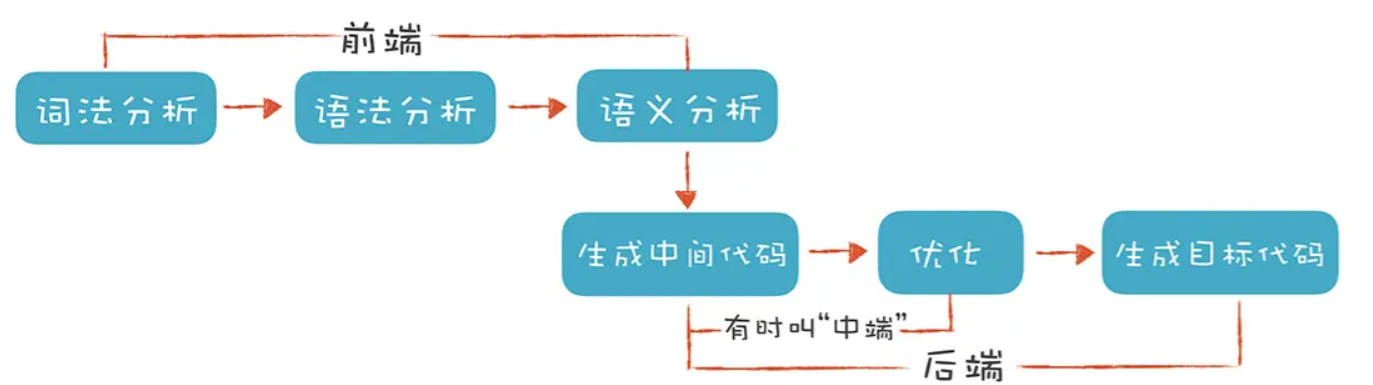
\includegraphics[scale=0.4]{pics/font1.png}
    \caption{編譯器架構}
    \label{p}
\end{figure}
    

编译器的“前端”技术分为词法分析、语法分析和
语义分析三个部分。
而它主要涉及自动机和形式语言方面的基础的计算理论。


\section{詞法分析}

詞法分析是將程式碼轉換為一個個的詞彙項目(Token)的過程。
像一段代碼中我们会识别出 if、else、int 这样的关键字,
main、printf、age 这样的标识符,+、-、= 这样的操作符号,
还有花括号、圆括号、分号这样的符号,以及数字字面量、字符串字面量等。
这些都是 Token。